\section{Предельное разрешение метода сухого электронно-лучевого травления резиста}

Исследование экспериментальных профилей показало, что при использовании пучка диаметром около 600 нм латеральное разрешение метода СЭЛТР, которое может быть оценено как ширина профиля на половине от максимальной глубины, составляет около 1 мкм. На основе разработанной модели процесса СЭЛТР можно предложить два пути увеличения разрешения данного метода.

Во-первых, латеральное разрешение метода СЭЛТР может быть увеличено за счет использования узкого высокоэнергетического пучка. Малый диаметр пучка позволит локализовать большинство разрывов молекул ПММА в центре линии, что вызовет интенсивную деполимеризацию, образование мономера и снижение вязкости резиста в этой области. В свою очередь, за счет высокой энергии пучка будет снижено число разрывов на краях линии, вызванных обратно отраженными электронами. При этом будет необходимо подобрать время экспонирования так, чтобы на момент остывания образца микрополости в центре линии оказались заполненными, а микрополости на краях -- остались незаполненными. Во-вторых, использование узкого низкоэнергетического пучка также может увеличить латеральное разрешение. При низкой энергии первичных электронов все разрывы полимерных молекул будут происходить вблизи центра линии за счет относительно небольшой глубины проникновения электронов. В этом случае микрополости будут формироваться только в ограниченной области вблизи центра линии, что исключит ``проседание'' краев линии.

Промоделированные профили, полученные методом методом СЭЛТР с латеральным разрешением, увеличенным обоими вышеописанными способами, приведены на рисунке~\ref{fig:DEBER_resolution}. При моделировании диаметр пучка был принят равным 10 нм, температура образцов -- 150~$^\circ$C/с, начальная толщина слоя ПММА -- 500 нм. Энергия пучка составляла 25 кэВ (высокоэнергетический пучок) и 5 кэВ (низкоэнергетический пучок), скорость охлаждения образцов -- 10~$^\circ$C/с. Моделирование проводилось для экспонирования вдоль одиночной линии, плотность тока экспонирования на единицу длины линии составляла 30 пА/см.

\begin{figure}[t]
	\begin{minipage}{0.48\textwidth}
		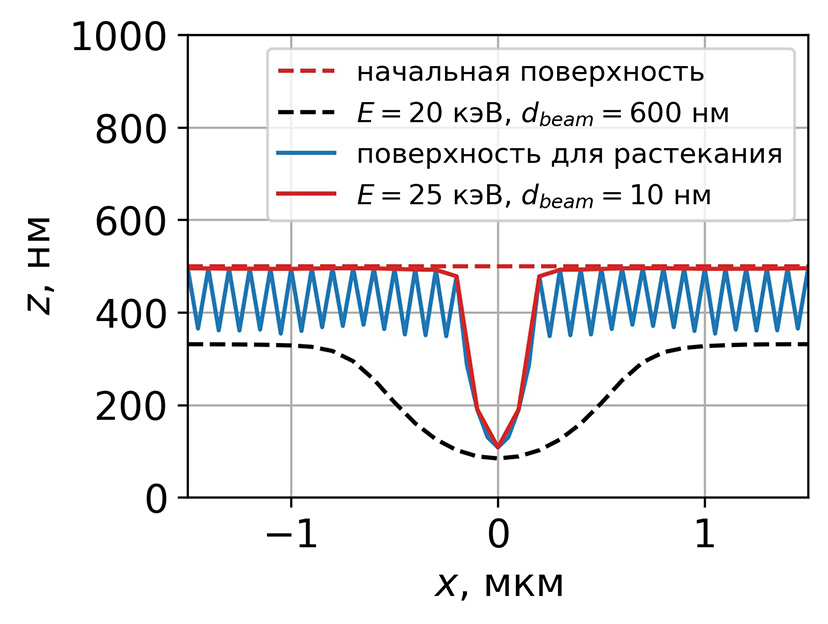
\includegraphics[width=\linewidth]{DEBER_resolution/resolution_25_um_200} \\
		\vspace{-28.7ex} \\ \text{\hspace{0em} a}) \\ \vspace{28.7ex}
	\end{minipage}
	\begin{minipage}{0.48\textwidth}
		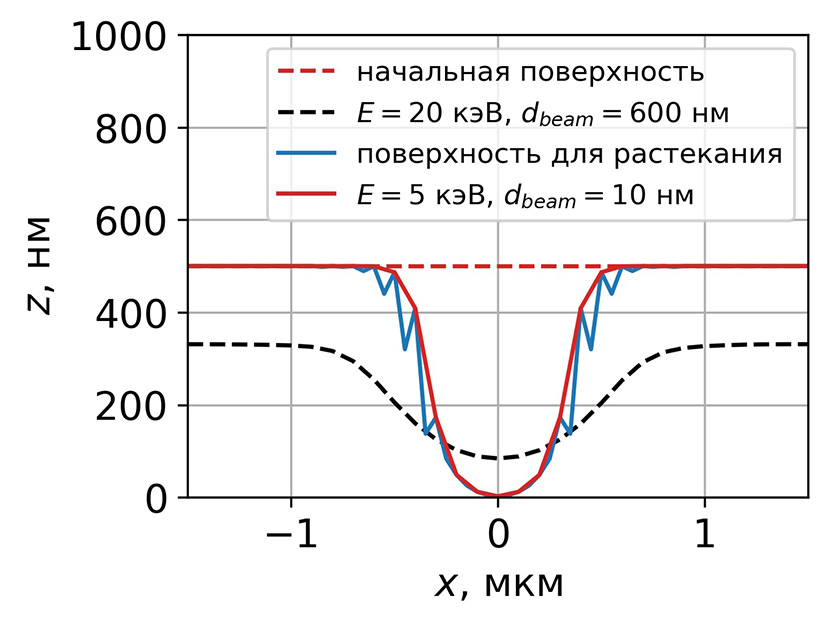
\includegraphics[width=\linewidth]{DEBER_resolution/resolution_5_um_200} \\
		\vspace{-28.7ex} \\ \text{\hspace{-0.1em} б}) \\ \vspace{28.7ex}
	\end{minipage}
	\vspace{-3.5em}
	\caption{Моделирование линий, полученных методом СЭЛТР с использованием узкого высокоэнергетического (25 кэВ, а)) и низкоэнергетического (5 кэВ, б)) пучка. Диаметр пучка составляет 10 нм, температура образцов -- 150~$^\circ$C/с, начальная толщина слоя ПММА -- 500 нм. Экспонирование производилось ``в линию'', плотность тока на единицу длины линии составляла 30 пА/см, скорость охлаждения образцов -- 10~$^\circ$C/с.}
	\label{fig:DEBER_resolution}
\end{figure}

Исходя из результатов моделирования, можно заключить, что использование узкого высокоэнергетического пучка способно обеспечить латеральное разрешение метода СЭЛТР до 300 нм. Было также установлено, что в этом случае толщина слоя ПММА в центре линии ограничена снизу значением около 100 нм, причиной чего является относительно большая средняя длина свободного пробега электронов при высоких энергиях, а также быстрое заполнение линии близлежащим резистом за счет процессов растекания. Использование узкого низкоэнергетического пучка, в свою очередь, обеспечивает латеральное разрешение всего лишь около 600 нм, однако, делает возможным полное травление резиста в центре линии за счет относительно небольшой средней длины свободного пробега электронов при низких энергиях. Следует также отметить, что во втором случае профиль полученной линии будет более устойчив к процессам растекания после экспонирования, поскольку вязкость резиста на краях линии будет оставаться практически на начальном уровне.

При этом в обоих вышеописанных случаях угол наклона профиля на полувысоте составляет около 70$^\circ$, что практически в три раза превышает максимальное значение угла наклона профиля в экспериментальных структурах \linebreak (около 25~$^\circ$).
